\chapter{Evaluation}
\label{chp:eval}

Evaluation is an important part of deciding whether SystemNaim achieved its aims \& goals. The following sections discuss: interconnect performance, program affinity and usability of SystemNaim, and attempt to gain insight into the issues or benefits produced by the tool.

\section{Interconnect Performance}
\label{sec:interconnect}

Calling a function implemented in hardware off-chip is not latency free. There will be some overhead latency associated with packaging the data to be sent over the channel, sending the data over the channel itself, and then repeating this process in order to return the data produced by the off-chip function back to the main FPGA. Therefore, it is of importance to measure this overhead so that we can gauge the efficiency of the interconnect hardware that was designed for SystemNaim.

Since the decision was made to implement an SPI communication channel for the final product, we had to into consideration the SPI clock speed used by the system. On an SPI channel, a single bit is sent on every cycle of the SPI clock meaning it takes 32 SPI Clock cycles to send single 32-bit integer. Increasing the SPI Clock speed allows for a higher performing channel, which is able to send data in a shorter period, however, this increase comes at the cost of reliability. This section explores the effect of the SPI Clock rate on a test system. We will attempt to prove that increasing the clock speed does reduce the total overhead, but will also investigate the overhead added from the interconnect to the latency of the system.

\subsection{Mathematical Model for Overhead Latency}

In order to find out how much of the latency of a multi-FPGA system, created in SystemNaim, can be attributed to the interconnect, we must first devise a model that can tell us what data needs to be gathered. At it's most simple, we can model the latency of a system as the sum of the time taken to perform the actual processing i.e. the code that the user entered into the tool, and the time taken to encode, transmit, receive, and decode the data across the SPI channel i.e. the overhead. \autoref{eqn:tot_sys_latency}, shows the mathematical equivalent of the previous statement.

\begin{equation}
    L_{sys} = L_{processing} + L_{overhead}
    \label{eqn:tot_sys_latency}
\end{equation}

In order to find $L_{processing}$ from \autoref{eqn:tot_sys_latency} we make the following assumption: the total processing time, in cycles, for a multi-FPGA system is the same as a single FPGA system where both the off-chip function and on-chip function, from the former system, are run in parallel. In essence, if we measure the latency of a system that has been created on a single FPGA using SystemNaim's “split” keyword then we can assume the total latency of this system is equal to $L_{processing}$ for a multi-FPGA system where “split” has been replaced with “split-fpga”.

Before we continue an important side note, $L_{rest}$ will refer to the latency caused by the processing outside the function call i.e. the processing before and after the function call. We can assume this because SystemNaim generates the exact same hardware in both the single FPGA and multi-FPGA case before and after the function call. Furthermore, for simplicity the single FPGA system with parallel hardware will be called the Multi-Thread Single Chip (MTSC) system, as it denotes parallel computation on a single chip, likewise, the multi-FPGA system will be referred to as the Multi-Thread Multi-Chip (MTMC) system. 

We can prove that $L_{processing} = L_{MTSC}$, where $L_{MTSC}$ is the total latency for an MTSC system, if we place the following constraint on the system: all parallel functions in the system must have the same latency.

\autoref{fig:multi_func_call} is a diagram representing the program path for a multi-function call in an MTSC system. As can be seen the total latency $L_f = max(L_1,L_2)$, however with our constraint $L_1 = L_2$, and thus we can simplify to \autoref{eqn:fcl_2}. \autoref{fig:multi_fpga_call} shows a similar diagram for the MTMC case. Assuming both functions are the same and that $L_{I1} > 0 \text{and} L_{I2} > 0 $ then equations \ref{eqn:mtmc_latency_start} to \ref{eqn:mtmc_latency} hold. 

\begin{align}
    &L_{f\_MTSC} = L_1 \label{eqn:fcl_1} \\
    &L_{MTSC} = L_{rest} + L_1 \label{eqn:fcl_2}
\end{align}

\begin{align}
    &L_{f\_MTMC} = max(L_1 + L_{I1} + L_{I2} , L_2) = L_1 + L_{I1} + L_{I2} \label{eqn:mtmc_latency_start} \\
    &L_{MTMC} = L_{rest} + L_1 + L_{I1} + L_{I2}  \\
    &L_{MTMC} = L_{MTSC} + L_{I1} + L_{I2} \\
    \therefore \; &L_{processing} = L_{MTSC} \label{eqn:mtsc_processing} \\
    \& \; &L_{overhead} = L_{I1} + L_{I2} 
    \label{eqn:mtmc_latency}
\end{align}

Given those results we prove that we can use the MTSC latency in the MTMC calculations. We also proved that the overhead was $L_{overhead} = L_{I1} + L_{I2}$, which represents the latency incurred by sending and receiving data over the channel and seems like a sensible representation of the overhead. Furthermore, \autoref{eqn:overhead_formula} show's that we can calculate the overhead latency by finding the difference between the latency of an MTMC and MTSC system, provided that they both call the same functions and have the same processing before and after the function call. In SystemNaim this is easily doable by switching the “split” keyword with “split-fpga”. 

\begin{align}
    &L_{MTMC} = L_{processing} + L_{overhead} \\
    &L_{overhead} = L_{MTMC} - L_{processing}  \\
    &L_{overhead} = L_{MTMC} - L_{MTSC}\label{eqn:overhead_formula}
\end{align}

\begin{figure}[!htb]
    \centering
    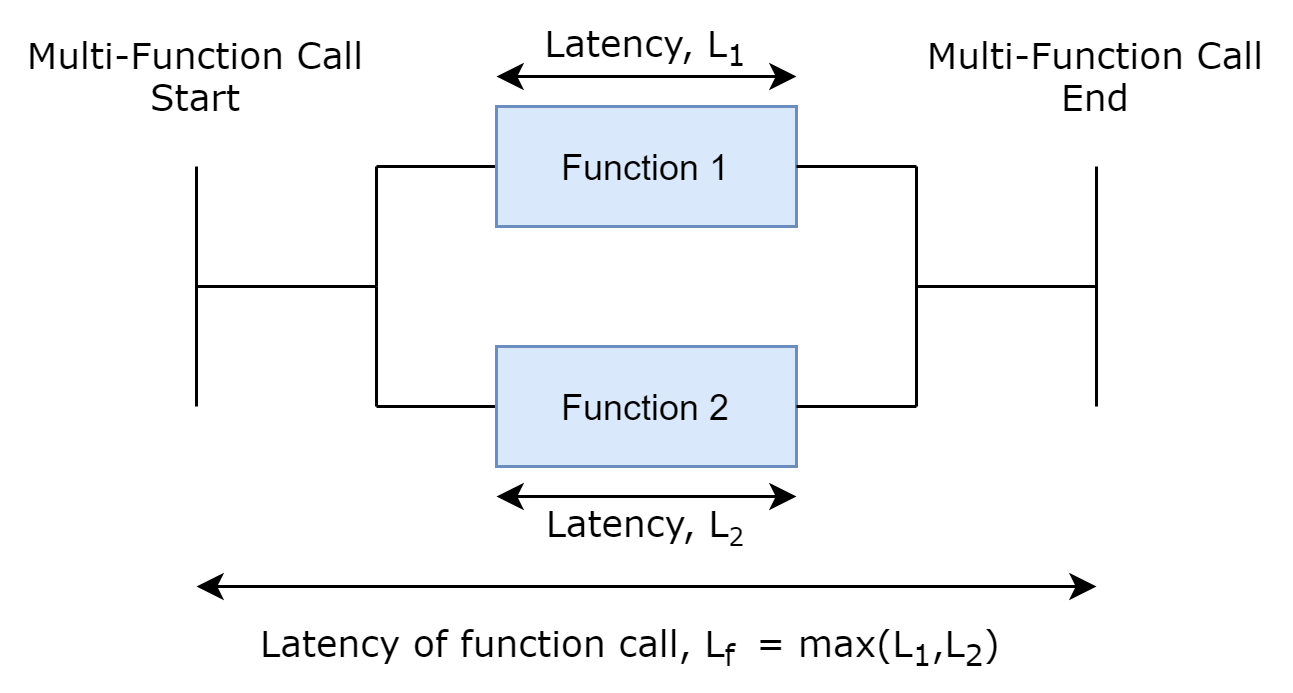
\includegraphics[width=0.9\textwidth]{05_evaluation/images/concurrent_latency.png}
    \caption{Latency of single FPGA multi-function call}
    \label{fig:multi_func_call}
\end{figure}

\begin{figure}[!htb]
    \centering
    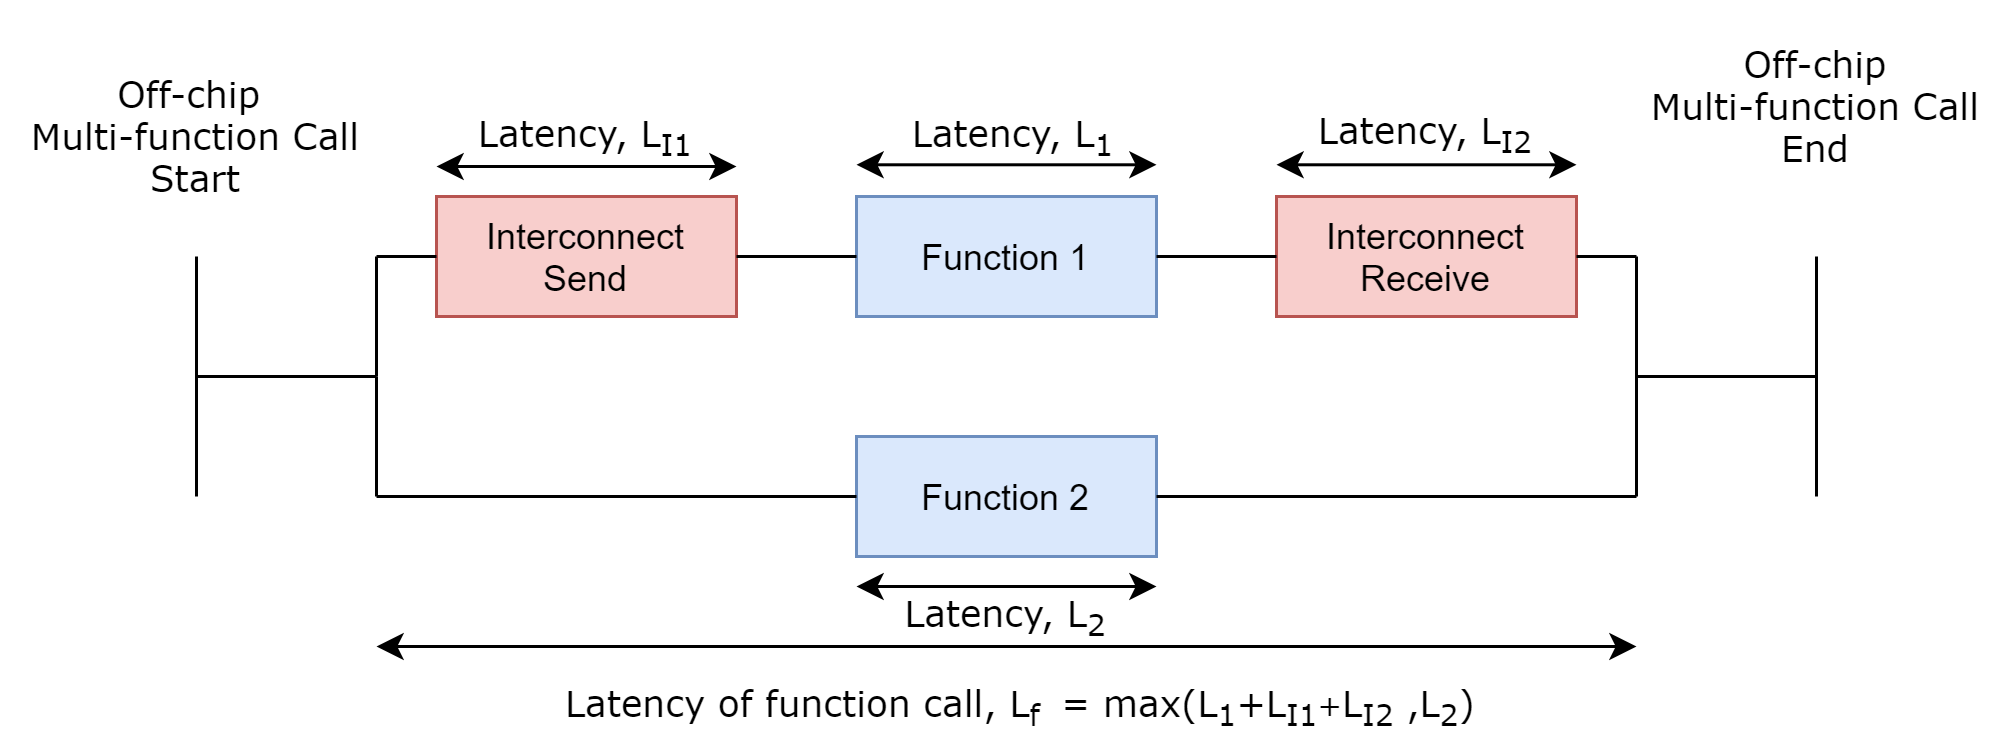
\includegraphics[width=0.9\textwidth]{05_evaluation/images/offchip_latency.png}
    \caption{Latency of multi FPGA multi-function call}
    \label{fig:multi_fpga_call}
\end{figure}

\subsubsection{Channel Bandwidth}
 
We can further dissect the overhead latency and split it into two parts. The transfer overhead, $L_{t\_overhead}$, which is latency cost incurred for transmitting and receiving data over a channel and the interconnect overhead, $L_{i\_overhead}$, which is the latency cost from encoding and decoding the data transmitted. Essentially, the latter part comes from the hardware designed specifically for SystemNaim, whereas the former is merely the limit of the channel. In an ideal world the interconnect overhead would be 0 and only the transfer overhead would exist. 

We can calculate the transfer overhead by knowing the rate at which data is transferred over the channel, and in the case of an SPI channel this is dependent on the SPI clock speed, $\mathit{SPI}_{clock}$. The SPI clock speed is different from the system clock speed, $\mathit{SYS}_{clock}$; both can be configured by the user but in our case we have a variable SPI clock speed and a static system clock speed at 50MHz.

Our SPI channel transfers data at 1 bit per SPI clock cycle, which is standard, however we're not interested in how long it takes for data to be transferred relative to the SPI clock. Instead, we would like to know how many system clock cycles it takes to transmit a single bit. We'll refer to this value as the channel latency, $L_{channel}$, and it can be calculated by dividing the system clock speed by the SPI clock speed. The resulting value has a unit of cycles per bit.

For SystemNaim, we know that any off-chip function call requires 128 bits of data to be sent over the channel. 96 bits (or 3 integers) are required to send the opcode, operand A and operand B, while the last 32 bits are for the data that needs to be returned to the main FPGA. Therefore, the formula for the transfer overhead, which is measure of how many clock cycles it takes to transfer all the data over a channel for an off-chip function call, is shown in \autoref{eqn:overhead}. 

\begin{equation}
    L_{channel} = \frac{\mathit{SYS}_{clock}}{\mathit{SPI}_{clock}} 
    \label{eqn:clock_speed}
\end{equation}

\begin{equation}
    L_{t\_overhead} = 128 * L_{channel}
    \label{eqn:overhead}
\end{equation}

\subsection{Test model}

With the maths and the modelling in place we can now begin testing the system to see if we can get an experimental value for the overhead and how it is affected by the SPI clock speed. For this test we use a program which calls 2 function, which are syntactically the same, and then exits. We first compile the program with both functions being called within a “split” block and test the latency of this MTSC system. Afterwards we test the same program, but we replace the “split” keyword with the “split-fpga” keyword, this will be the MTMC system. 

The MTMC system will be run multiple times with varying SPI clock speeds, and for each test we will compare the latencies between the MTMC and MTSC systems, compute the transfer overhead and find the interconnect overhead.

\subsection{Results}

\autoref{tbl:spi_clk_results} shows the data gathered, in accordance to testing methodology laid out above. It should be noted that the \textbf{Channel Latency} and \textbf{Est. Transfer Overhead} columns have been calculated using no gathered data. Both columns are dependent on the \textbf{SPI Clock (Hz)}, and the calculations for each can be found in Equation \ref{eqn:clock_speed} and \ref{eqn:overhead} respectively.

\autoref{fig:spi_clk_graph} is a summation of the important data from the table in the form of graph, thus making it easier to identify trends in the data.

\begin{sidewaystable}
    \centering
    \begin{threeparttable}
    \begin{tabular}{l|l|l|l|l|l}
    \textbf{SPI Clock (Hz)} & \textbf{Channel Latency} & \textbf{Latency (Cycles)} & \textbf{Overhead (Cycles)} & \textbf{Transfer Overhead} & \textbf{Interconnect Overhead} \\ \hline
     125,000               &  400                 &  52,918              &  52,794              & 51,200                &  1,594                                      \\
     250,000               &  200                 &  26,518              &  26,394              & 25,600                &  794                                        \\
     252,525\tnote{*}      &  198                 &  26,254              &  26,130              & 25,344                &  786                                        \\
     277,777\tnote{*}      &  180                 &  23,878              &  23,754              & 23,040                &  714                                        \\
     312,500               &  160                 &  26,532              &  26,408              & 20,480                &  5,928                                      \\
     347,222\tnote{*}      &  144                 &  23,892              &  23,768              & 18,432                &  5,336                                      \\
     500,000               &  100                 &  16,632              &  16,508              & 12,800                &  3,708                                      \\
     1,000,000             &  50                  &  8,382               &  8,258               & 6,400                 &  1,858                                      \\
     1,923,076\tnote{*}    &  26                  &  4,422               &  4,298               & 3,328                 &  970                                        \\
     5,000,000             &  10                  &  1,782               &  1,558               & 1,280                 &  278                                        \\
     8,333,333\tnote{*}    &  6                   &  1,122               &  998                 & 768                   &  230                                        \\
     12,500,000            &  4                   &  792                 &  668                 & 512                   &  156                                        \\
     25,000,000            &  2                   &  542                 &  418                 & 256                   &  162                                       
    \end{tabular}
    \begin{tablenotes}\footnotesize
        \item[*] These values for SPI clock speed are not factors of the system clock, and are actually irrational.
        \end{tablenotes}
    \end{threeparttable}
    \caption{Effect of SPI clock speeds on overhead latency}
    \label{tbl:spi_clk_results}
\end{sidewaystable}

\begin{figure}[!htb]
    \centering
    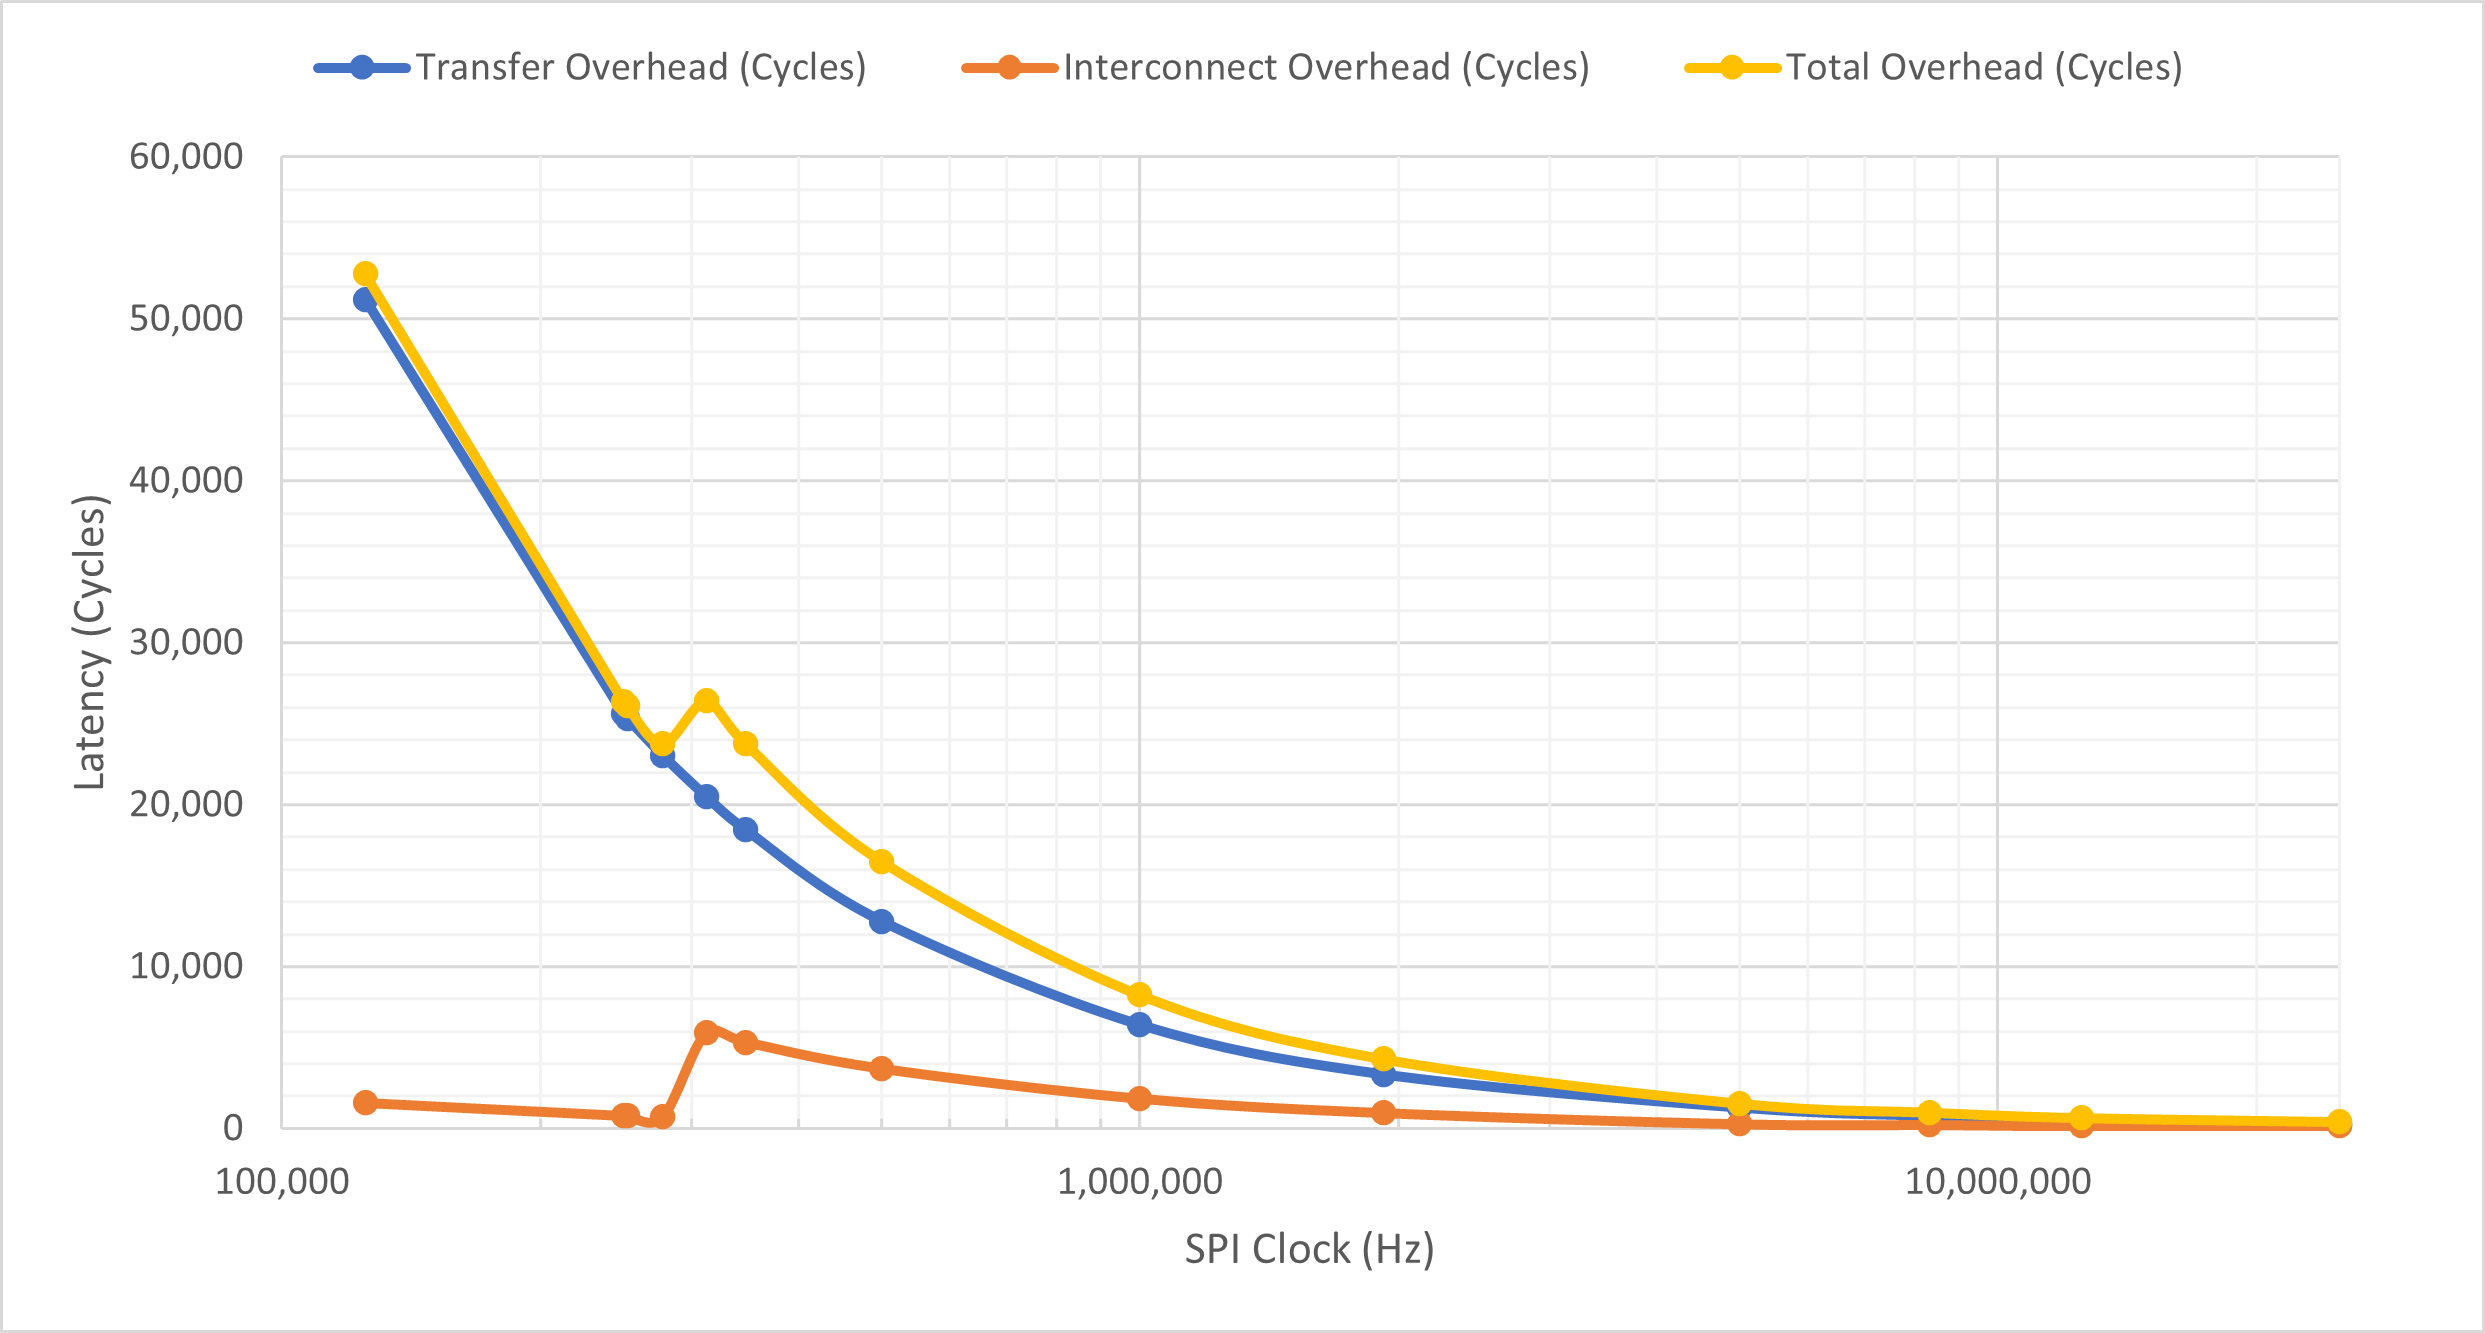
\includegraphics[width=0.9\textwidth]{05_evaluation/images/overhead_vs_spi_clk.png}
    \caption{Overhead Latency vs. SPI Clock Speed \textit{(Best case would be that the total overhead equals the transfer overhead)}} 
    \label{fig:spi_clk_graph}
\end{figure}


\subsection{Conclusions}

Generally speaking, we can conclude that as we increase the SPI clock speed the total overhead latency decreases, we can also deduce that the main proportion of the overhead is transfer overhead. This is supported by \autoref{fig:spi_clk_graph}, and was the result we intended for this investigation to prove. However, there are a few interesting caveats to this conclusion that we cannot ignore. Firstly, while not shown on the graph or table, during testing it was found that setting the clock speed the values higher than 8MHz resulted in increased channel instability. Tests would occasionally fail to complete with transactions not being detected by either the on-chip or off-chip interconnect, the higher the clock speed the more likely this phenomenon would occur.

This instability may have been caused by the physical components of the channel not being able to accurately keep up with these speeds. For the final product GPIO pins on both FPGAs were connected using breadboard jumper cables, which aren't intended to be used for data communication. Potentially, at clock speeds of 8MHz and above, the GPIO pins were not able to go from high to low, and vice versa, fast enough to generate a detectable clock on the child FPGA. The fault could also lie with the SPI core and the FPGA hardware. The SPI core takes in the main system clock, generates the SPI Clock and transmits that signal to a GPIO pin. Therefore, there may be an issue between the pin and the FPGA hardware. Unfortunately, there's no way to be certain of the cause, and instead we can only conclude that speeds above 8MHz result in unreliable performance. 

The more interesting result from the gathered data, however, comes from the trend of the \textbf{Interconnect Overhead}. While it would be expected that the latency from the interconnect would be generally static, with only minor fluctuations since the task of encoding data should be uniform, what we see instead is a generally decreasing trend except for a steep rise in latency at 312,500Hz. This behaviour, however, makes complete sense given the design of the interconnect and is a consequence of the SPI channel only allowing the master to initiate transactions. 

As explained in \autoref{sec:impl_interconnect}, the child FPGA cannot indicate to the parent FPGA when it has completed processing its off-chip function. Therefore, in order to receive the return data the parent FPGA must continuously send polling transactions on the SPI channel. Because of this, when the off-chip function is complete, and it passes the result to the SPI slave core, the core must wait for the current polling transaction to finish before the next one starts, and then it can send the valid return data. Therein lies the issue, the wait for a current transaction to finish.

The worst case for this scenario is if the slave SPI core has to wait for a full transaction, minus one cycle, to complete before it can send its data. At lower clock rates this can take thousands of cycles, more specifically $32 * L_channel$ cycles, since each transaction consists of 32 bits. Furthermore, how close the end time of an off-chip function is to the end of any given polling transaction is dependent on both the SPI clock speed and the latency of the function itself, therefore it becomes incredibly difficult to avoid the worse case scenario and the interconnect overhead becomes stochastic in nature. However, we can minimize the interconnect overhead by increasing the SPI clock speed, as this reduces the number of system cycles it takes for a polling transaction to finish and thus also the number of system cycles the slave SPI core has to wait in the worse case scenario.

In conclusion, we should try to maximize the SPI clock speed as this reduces the transfer overhead, and minimizes the worst case for the interconnect overhead, thus, increasing the performance of the MTMC system.

\section{System Performance}
\label{sec:sys_perf}

Now that we have established that higher SPI clock speeds, and also higher channel bandwidths, reduce the total overhead associated with calling a function off-chip, we can start to explore what kind of programs can exploit the benefits of a multi-FPGA system the best. In general, FPGAs are mainly used for their ability to exploit parallelism in programs, and the motivation for using multiple FPGAs in tandem is to access more resources (LUTs, BRAM, DSPs etc.). Therefore, it stands to reason that the best programs to run on a multi-FPGA system are one which can have large parts of the processing run in parallel but also require a large amount of resources.

Considering the limitations of SystemNaim it would be difficult for us to write programs which take up a large percentage of an FPGAs resources, however, we can investigate how well we can exploit a program's affinity for parallelism and how the same program performs on a single FPGA system versus a multi-FPGA system. Ideally, we will be able to prove that as program latency increases the percentage contribution of the interconnect overhead to the total latency will decrease, thus, giving more credence to using a multi-FPGA system.

\subsection{Test Model}

The model for this investigation is relatively straightforward. We will write a numerical integration program and using SystemNaim, run the program on three different systems. The first will be a full sequential program with no parallelism, the second will exploit the parallelism of the program, but all processing will happen on a single FPGA, the final system will be a multi-FPGA one, which will also exploit the parallelism of the program but will also perform some processing on a second FPGA.

Borrowing from the previous investigation each system will have a short-hand to make them easier to identify. The sequential system will be the Single-Thread Single Chip (STSC) system, the single FPGA system with parallelism will be the Multi-Thread Single Chip (MTSC) system and finally the multi-FPGA system will be the Multi-Thread Multi-Chip (MTMC) system.

The program that we will be running will contain loops that run for a fixed number of iterations. As we vary the number iterations, we will measure the latency of each system at each step and compare the results. Furthermore, we will dissect the MTMC latency into processing latency and overhead, where the overhead is a measure of the cost incurred, in cycles, for perform part of the processing off-chip.

As a final note, the SPI core in this investigation will be set at 5MHz or 10\% of the system clock. This decision was made in order minimize channel latency, while maintaining reliability.

\subsection{Numerical Integration Program}

The numerical integration method that we decided to implement was the Composite Simpson's rule, which is shown in \autoref{eqn:comp_simp}. What makes this specific implementation interesting to us are the two sums, $s_1$ and $s_2$. These sums can be easily setup so that they are computed in parallel when implemented in SystemNaim. All that is needed is to make functions of each sum and call them within a “split” or “split-fpga” block to produce either an MTSC or MTMC system respectively. $n$, is also chosen by the user, and we can increase that to increase the number of total iterations the program must make.

Unfortunately, since a function in SystemNaim can only have two numerical inputs there are some limitations on the program. The first is that $a$, the lower bound of the integral will be a compile-time constant, thus, unmodifiable during runtime. The second is that both functions will have knowledge of what $f(x)$ is at runtime, and will make calls to a function in software which computes the value of $f(x)$. Each of these calls in software will create a module in hardware, resulting in two hardware modules which compute $f(x)$. This, however, is necessary for the parallelism and will allow for some interesting analysis that will be explored later on.

The final issue is unrelated to the two input problem, but is due to SystemNaim not supporting floats. Only integers are supported and to ensure we produce valid results, care has been taken in order to choose $a$, $b$, $n$, and $h$ such that no decimal values are produced during operation.

Overall, none of the three issues disrupt the purpose of the investigation at hand, which focuses on how the latency of the systems are affected as we increase the number iterations the program has to run. However, in the interest of a fair and open investigation it was deemed important to include them.

\begin{align}
    & s_1(f(x),n,a,h) = 2 \sum_{j=1}^{n/2-1}f(x_{2j}) \text{, where } x_j = a + jh \\
    & s_2(f(x),n,a,h) = 4 \sum_{j=1}^{n/2}f(x_{2j-1}) \text{, where } x_j = a + jh \\
    &\int_{a}^{b} f(x) dx \approx \frac{h}{3} \Big[ f(x_a) + s_1(f(x),n,a,h) + s_2(f(x),n,a,h) + f(x_b) \Big] \text{, where } h = \frac{b-a}{n}  \label{eqn:comp_simp}
\end{align}

\subsection{Results}

\autoref{tbl:system_results} shows the results of the investigation. \autoref{fig:latency_v_iter} shows the same data but in the form of graph in order to be able to identify trends more easily.
Finally, \autoref{fig:overhead_percent} shows the percentage contribution of the overhead to the MTMC latency, however, this graph needs a slight amount of justification before we can draw conclusions from it.

The investigation has been designed in such a manner that the MTSC and MTMC systems are exploiting the same amount of parallelism in the program and are preforming the same amount of processing. The only difference is that the MTMC must also go through the trouble of calling a function off-chip, which has been proved to incur a latency cost. Therefore, we assume that the processing latency i.e. the amount of cycles spent executing the code that the user entered into the tool, are the same for both systems. Thus, the difference between the two latencies is the cost incurred to call a function off-chip and is therefore the latency. This was much more rigorously proved in the previous investigation but the reasoning above provides an adequate platform for this section.

Finally, by comparing the MTSC latency and the calculate overhead we can guage what percentage of the total latency of the MTMC system was due to the off-chip function call and thus evaluate whether the jump from single FPGA to multi-FPGA is worth the latency cost. 

\begin{sidewaystable}
    \centering
    
    \begin{threeparttable}
    \begin{tabular}{l|l|l|l|l|l}
    \textbf{Iterations ($n$)} & \textbf{STSC Latency} & \textbf{MTSC Latency} & \textbf{MTMC Latency} & \textbf{Overhead} & \textbf{STSC to MTMC Latency Reductions}\\ \hline
     200        & 2,572               & 1,370                 & 2,839                 &  1,469         &    -10.38\%    \\
     400        & 5,072               & 2,670                 & 4,215                 &  1,545         &    16.9\%    \\
     600        & 7,572               & 3,970                 & 5,591                 &  1,621         &    26.1\%    \\
     800        & 10,072              & 5,270                 & 6,967                 &  1,697         &    30.1\%    \\
     1000       & 12,572              & 6,570                 & 7,999                 &  1,429         &    36.4\%    \\
     1200       & 15,072              & 7,870                 & 9,375                 &  1,505         &    37.8\%    \\
     1400       & 17,572              & 9,170                 & 10,751                &  1,581         &    38.8\%    \\
     1600       & 20,054              & 10,470                & 12,127                &  1,657         &    39.5\%    \\
     1800       & 22,572              & 11,770                & 13,503                &  1,733         &    40.2\%    \\
     2000       & 25,072              & 13,070                & 14,535                &  1,465         &    42.0\%    \\                                 
    \end{tabular}
    \begin{tablenotes}\footnotesize
        \item Latencies are measured in cycles
        \end{tablenotes}
    \end{threeparttable}
    \caption{Effect of Program iterations on total latency}
    \label{tbl:system_results}
\end{sidewaystable}

\begin{figure}[!htb]
    \centering
    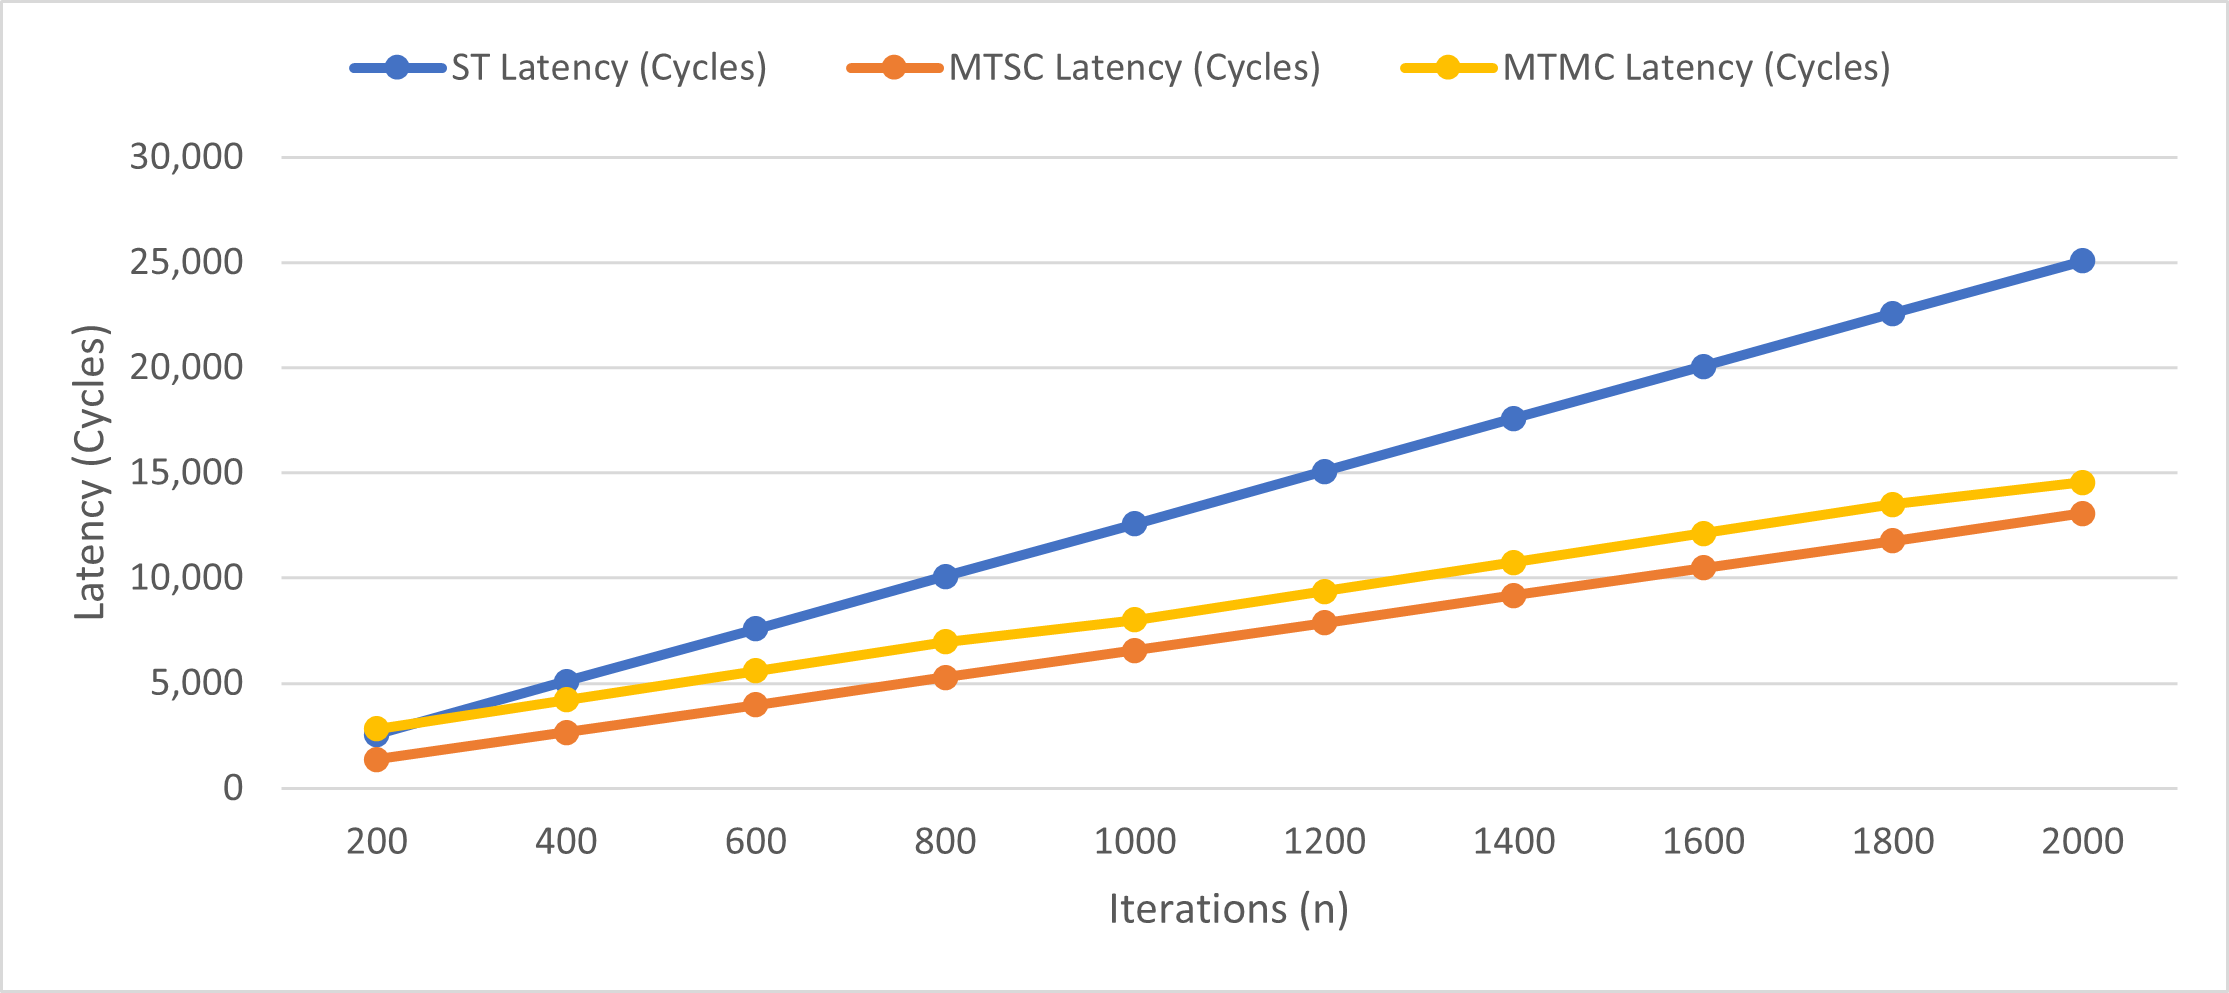
\includegraphics[width=0.9\textwidth]{05_evaluation/images/latency_vs_iter.png}
    \caption{Latencies of different systems as iterations of program increase \\ \textit{STSC = Single Thread Single Chip, MTSC = Multi Thread Single Chip and MTMC = Multi Thread Multi Chip }}
    \label{fig:latency_v_iter}
\end{figure}

\begin{figure}[!htb]
    \centering
    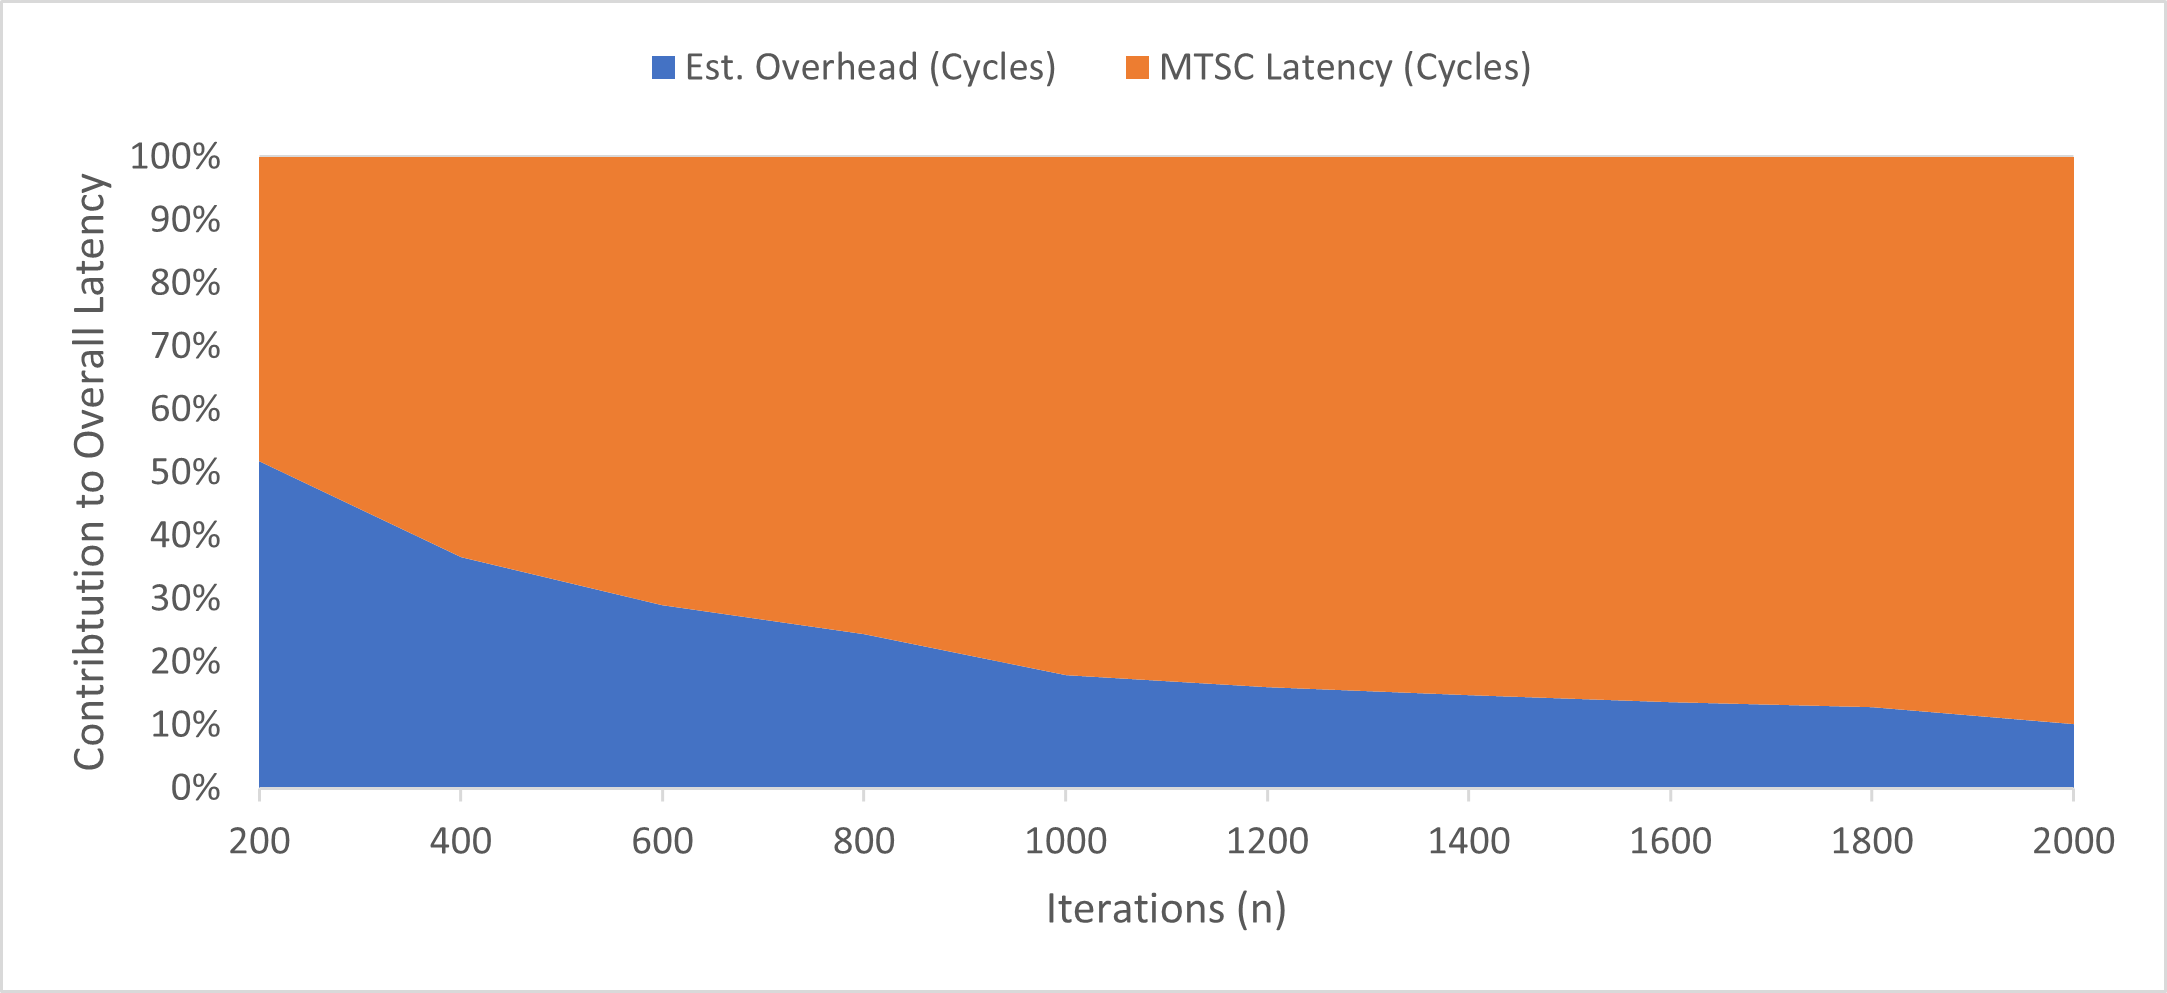
\includegraphics[width=0.9\textwidth]{05_evaluation/images/overhead_percentage.png}
    \caption{Percentage contribution of overhead to total latency}
    \label{fig:overhead_percent}
\end{figure}

\subsection{Conclusions}

Our main conclusion from this investigation is that as we increase the number of iterations the program has to perform, the overhead in the MTMC system contributes less to the overall latency. This claim is supported by \autoref{fig:overhead_percent}, as you can see that with a declining trend in the percentage contribution from the overhead as iterations increases. What we can then conclude is that MTMC systems in which the off-chip function has a large processing latency will perform more equally to their MTSC equivalent systems, therefore, it advised to users of SystemNaim to code their programs in such a way that the designated off-chip function has as much processing time as possible i.e. it has a loop with a large bound within it. If the users fails to do so, they might end up with an MTMC system that performs worse than its STSC counterpart, as can be seen in \autoref{fig:latency_v_iter} when steps = 200. 

Further, by observing the relationship between the latency of the STSC and MTSC system in \autoref{fig:latency_v_iter}, and \autoref{tbl:system_results}, we can see that exploiting the parallelism in the program gave us approximately 48\% reduction in latency, this is due to the fact that there were two sums, $s_1$ and $s_2$, that we calculated in parallel. We can extrapolate from this and say that if you had a program which had three segments which could be run in parallel you would be able to achieve a 3x speed up, and as you increase the number of parallel segments, be they a loop or some other part of the program, you can achieve further performance increases. Therefore, it is advisable to users of SystemNaim to analyse, and potentially rewrite, to exploit as much parallelism as possible while also offloading as much processing to the child as possible.

However, a user must be careful in where they place their off-chip function call. If placed within a loop the overhead does not occur once, but rather it occurs for remote function call. Now this may not be too much of a concern if the processing latency of the off-chip function hardware is high relative to the overhead, but it would be preferable to try and reduce the number of calls to off-chip functions to reduce the contribution the overhead latency makes to the total latency of the system.

From the \autoref{tbl:system_results}, we can see that as we increase the number of iterations the MTMC system approaches the same percentage reduction latency as the MTSC system, compared to the STSC system. This 48\% reduction represents the maximum performance gain we can get from running the program as a multi-FPGA system, and therefore a 42\% reduction, which is what is achieved when we run the system at steps = 2000, proves that SystemNaim is able to create a multi-FPGA system that lets the user achieve a latency decrease without the overhead outweighing the performance gains, which is a major contribution specified in \autoref{sec:contributions}. 

\subsection{Interconnect Latency Variation}

One thing of note, is that the stochastic nature of the interconnect is likely due to the polling issue mentioned in the previous investigation, however as can be seen in \autoref{tbl:system_results}, the overhead tends to be centred around an average value of 1,570 cycles which is close to the overhead measured in \autoref{tbl:spi_clk_results} for the 5MHz SPI clock, the same speed as the SPI clock in this investigation. The range of the measured overheads is 304 cycles, thus, the total overhead latency will be at most 20\% away from the average. This can be seen as an issue for programs with low latencies, but as mentioned above those programs wouldn't be advisable for SystemNaim. 

\subsubsection{Too few resources for MTSC}

A final thing that can be discussed is the necessity for the both the MTSC and MTMC systems to instantiate two hardware modules to calculate $f(x)$. While not the case in this investigation, the hardware module for $f(x)$ may potentially be very resource intensive, specifically, mathematical functions tend to use a lot of DSPs. In the case where a single FPGA may not have enough DSPs, or any other resource, to instantiate two modules to compute $f(x)$, you would no longer be able to create an MTSC system. As an example if each $f(x)$ module took 3 DSPs and our FPGA only had $5$, we would be one short of the required $6$. The user's options would then either be to run the system sequentially, and achieve the results of an STSC system, or it would be to instead use multi-FPGA solution and utilize an MTMC system. Therefore, SystemNaim can solve the issue of a user having FPGA boards with too few resources to implement their design. This would be a real-world motivation for using a multi-FPGA system and thus provides credence to the purpose of SystemNaim.

\section{Usability}
\label{sec:usability}

One of the major motivations of SystemNaim is increasing the accessibility of multi-FPGA systems to people who may not be very hardware proficient. The way we have tried to tackle this goal is by creating a HLS tool which requires knowledge of C90 and basic programming constructs, therefore allowing the tool to be used by a larger group. 

In order to illustrate the usability of the tool we will go through a design example, where we create a multi-FPGA system in SystemNaim,  and then perform a qualitative comparison to creating a similar system but purely in Quartus II using only SystemVerilog and the IP catalog.

\subsection{Design Example: Numerical Integration}
\label{sec:design_example}


For this design example we have decided to show how we implemented the Composite Simpson numerical integration method that was used in the investigation in \autoref{sec:sys_perf}.


\subsubsection{Writing the program.}

The first step for any user would be to write the C code. For this example in particular this took around 15 minutes and the original C code Listing \ref{lst:c_simp_st}. The user must then tell the tool which functions they wish to run in parallel, by encapsulating those functions inside either a “split” or “split\_fpga” block. An example of this is shown in Listings \ref{lst:org_to_par} and \ref{lst:par_to_off}. The case when a user decides to use “split\_fpga” is of the primary focus of this section, therefore, from now on we assume that decision has been taken. \textit{Note: The first function in a “split\_fpga” block is the one that will be run on the child FPGA.} 

Currently, the tool will need to be compiled by the user, however, to make this process easier a Makefile has been provided. \autoref{fig:dir} shows the directory structure for the SystemNaim tool. Running the command “make” while in “Working Directory” will compile the tool.

A test bench folder, “tb”, is also provided. However, this was mainly used for testing during development and most programs created by SystemNaim should not need to be tested. If a user does wish to test their program they will need to install Verilator, and it should be noted that programs which use the “split\_fpga” construct are unable to be tested. Instead, it is recommended to test the same program using the “split” construct instead.

\begin{figure}
\centering
\begin{minipage}{0.47\textwidth}
    \dirtree{%
    .1 Working Directory.
    .2 bin.
    .2 include.
    .2 out.
    .2 hardware\_files.
    .3 parent\_fpga.
    .4 sysNaim\_spi\_handler.sv.
    .4 sysNaim\_master\_mux.sv.
    .4 sysNaim\_instr\_encoder.sv.
    .3 child\_fpga.
    .4 sysNaim\_spi\_slave\_handler.sv.
    .4 sysNaim\_slave\_muxsv.sv.
    .4 sysNaim\_instr\_decoder.sv.
    .3 platform\_designer.
    .4 parent\_cpu.qsys.
    .4 child\_cpu.qsys.
    .2 src.
    .2 tb.
    .2 Makefile.
    }
\end{minipage}
\caption{Current base SystemNaim directory.}
\label{fig:dir}
\end{figure}

Once the code has been properly modified, the user can then pass the program files as argument to the tool, which at this stage is an executable, and in the “out” folder they will find the output Verilog files which describe their program as a set of hardware modules.


\subsubsection{Implementing the system in Quartus.}

The next few parts require the use of Quartus Prime, Intel's Platform Designer and the NIOS II system. Pre-made files are provided for the Platform Designer, so the user isn't required to have an in depth understanding of that tool. However, the ability to assign pins and create a top level file in Quartus will be needed.

The following instructions will also be relatively brief, as they are not intended to be used as a guide but rather to give an overview of the complexity of creating a system. Most of these steps are pretty simple, however they can appear to be complicated to a first time user of Quartus Prime since it is a very bloated and non-self-explanatory tool. 

The first thing a user will need to do is create a Quartus project and select their FPGA. They will then need to create a top level clock and assign names to 4 of the GPIO pins on their FPGA. Any names will work, but we recommend the following: SPI\_MISO, SPI\_MOSI, SPI\_SS, SPI\_CLK. Add these to the top level file, preferably a block design file (shown in \autoref{fig:qp_pins}), and they will be used later.

\begin{figure}[!htb]
    \centering
    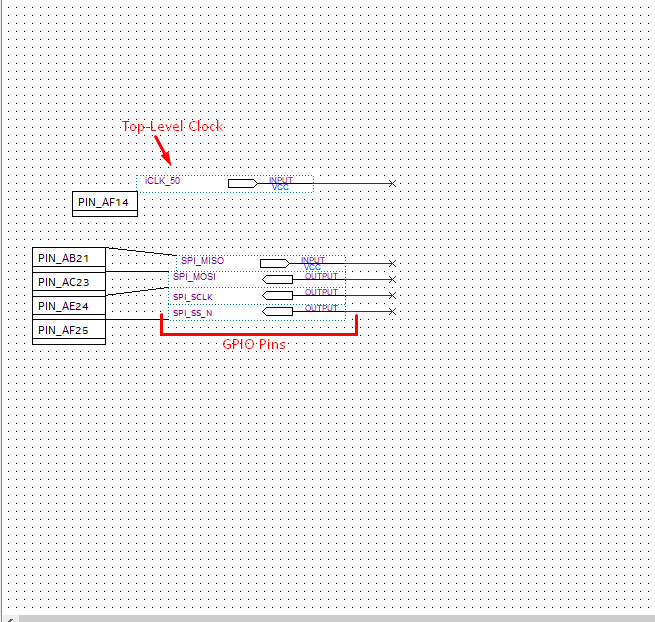
\includegraphics[width=0.9\textwidth]{05_evaluation/images/just_pins.png}
    \caption{Quartus Prime: Top Level BDF w/ GPIO Pins and System Clock }
    \label{fig:qp_pins}
\end{figure}

\subsubsection{Platform Designer}

Now we move onto the Platform Designer. This tool allows you to quickly connect up hardware modules and will allow the user to connect their custom hardware with the NIOS II processor. This processor will act as a controller for our hardware, and will tell it when to start operating as well as provide it the initial inputs. To streamline the process of creating a new NIOS II system, two “.qsys” files have been provided. 

When you open up Platform Designer, you will be prompted to select which “.qsys” file you want to open. These files save the design you have been working for, but also allow us to distribute pre-made systems. Open up the “parent\_cpu.qsys” file, and you should see something similar to \autoref{fig:pd_start}.

\begin{figure}[!htb]
    \centering
    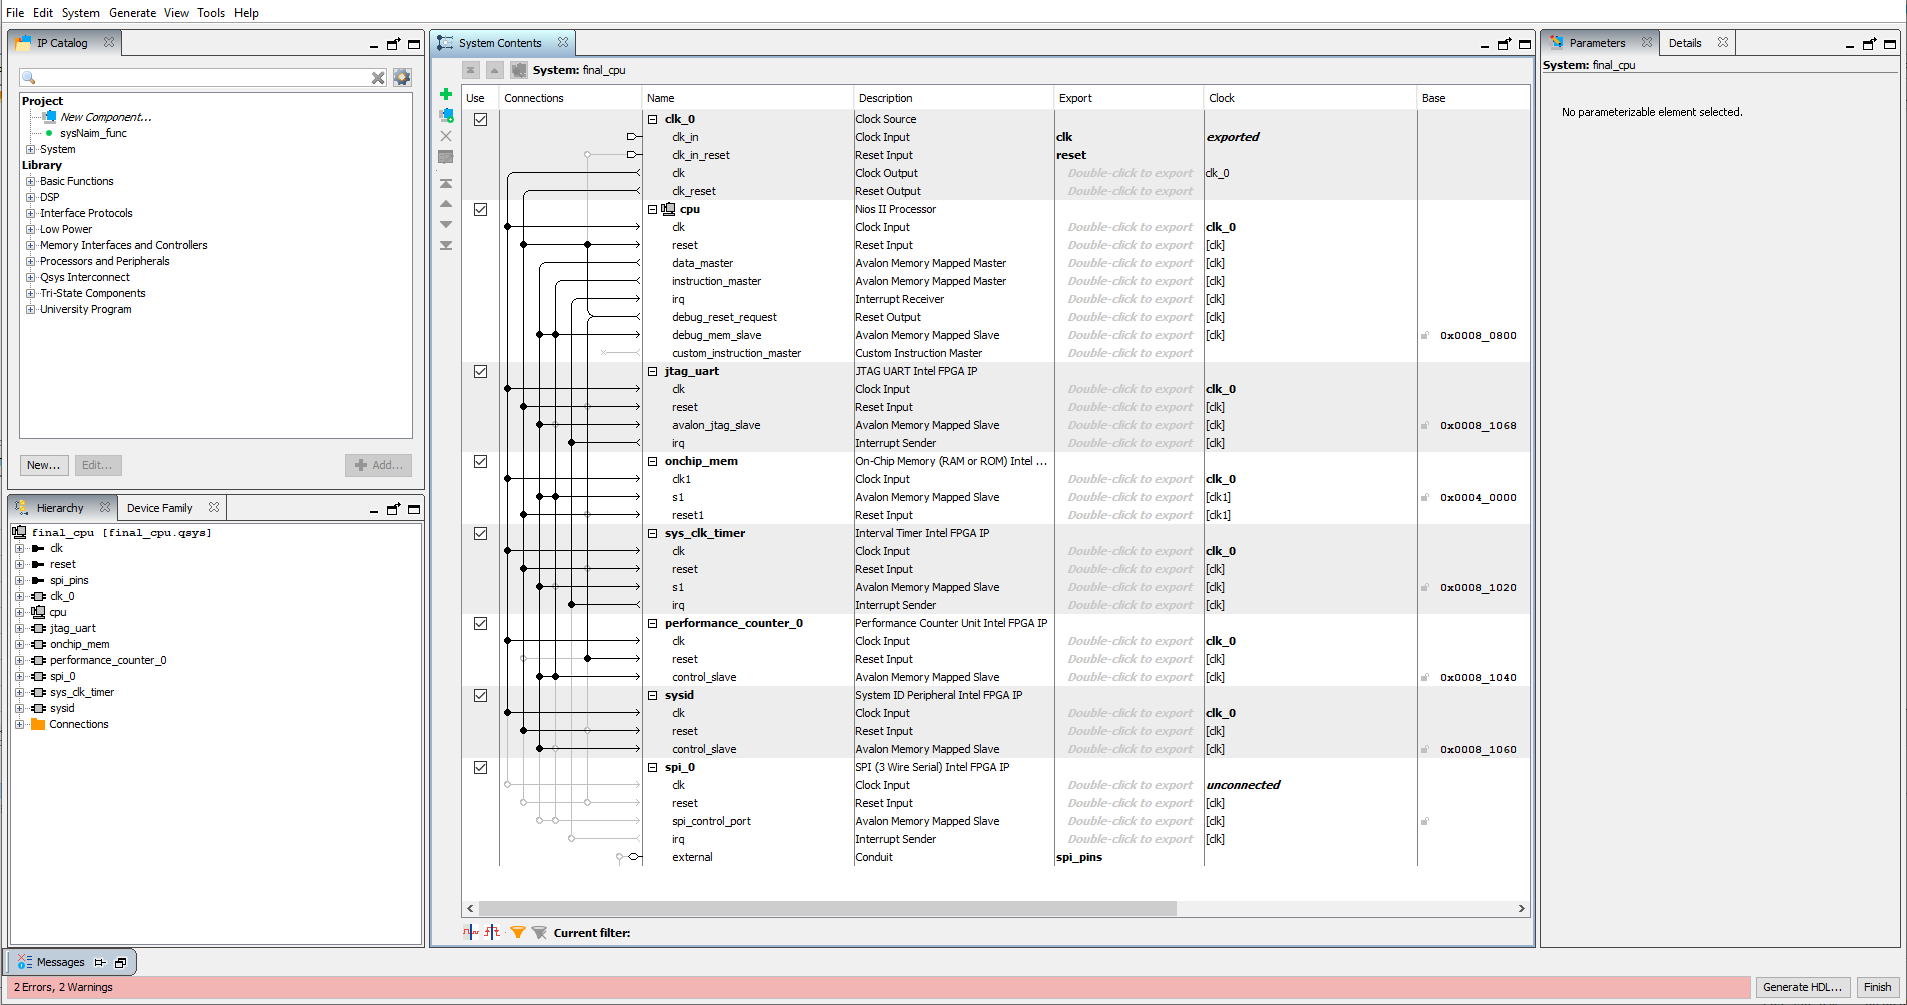
\includegraphics[width=0.9\textwidth]{05_evaluation/images/pd_no_module.png}
    \caption{Platform Designer: System before we add custom hardware.}
    \label{fig:pd_start}
\end{figure}

The user can then add their own custom hardware to the system. In order to do so, they need to click “New...” in the IP Catalog, which results in another window being opened: the Component Editor. In the first tab of this window, “Component Type”, a user can specify the name of their module. More importantly, they need to go to the “Files” tab to include the files generated by SystemNaim. In this tab, they need click “Add File...” under “Synthesis Files” and select all the files generated by SystemNaim in the “out” folder\footnote{It is possible to select only the files needed by the “sysNaim\_host\_top.sv” file, as well as the files needed by its dependencies. But this might get tedious for larger systems.} and then also add the files in the “hardware\_files/parent\_fpga” folder. The user must then find the “sysNaim\_host\_top.sv”, in the file list, and set its attribute to “Top-level file”. 

\begin{figure}[!htb]
    \centering
    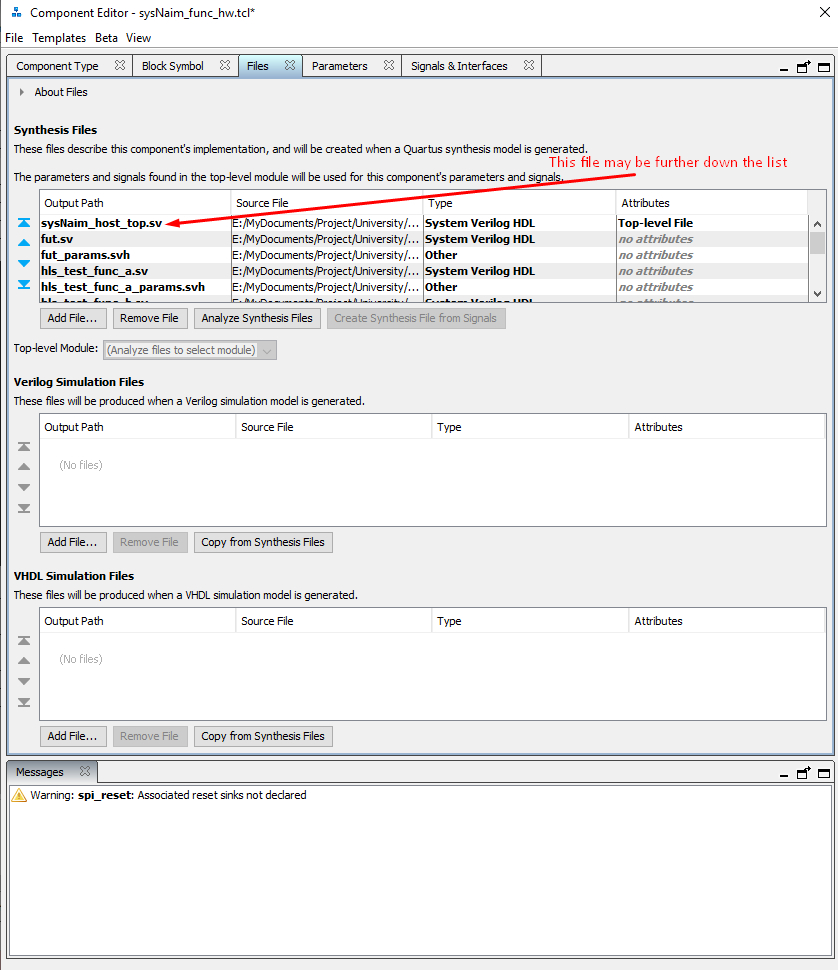
\includegraphics[width=0.9\textwidth]{05_evaluation/images/pd_sys_files.png}
    \caption{Platform Designer: Generated files added to the component editor.}
    \label{fig:pd_files}
\end{figure}

The user can then click “Analyse Synthesis Files”, if this step does not produce any errors they can move onto the “Signals \& Interfaces” tab. This tab will likely be a mess, and it is recommended to delete all pre-existing entries on the left sub-window. The user will then need to add the interfaces and signals until it looks like \autoref{fig:pd_interfaces}. The user should take extra note of the text in grey next to each signal and interface as this denotes type and is extremely important to get correct for proper synthesis.

\begin{figure}[!htb]
    \centering
    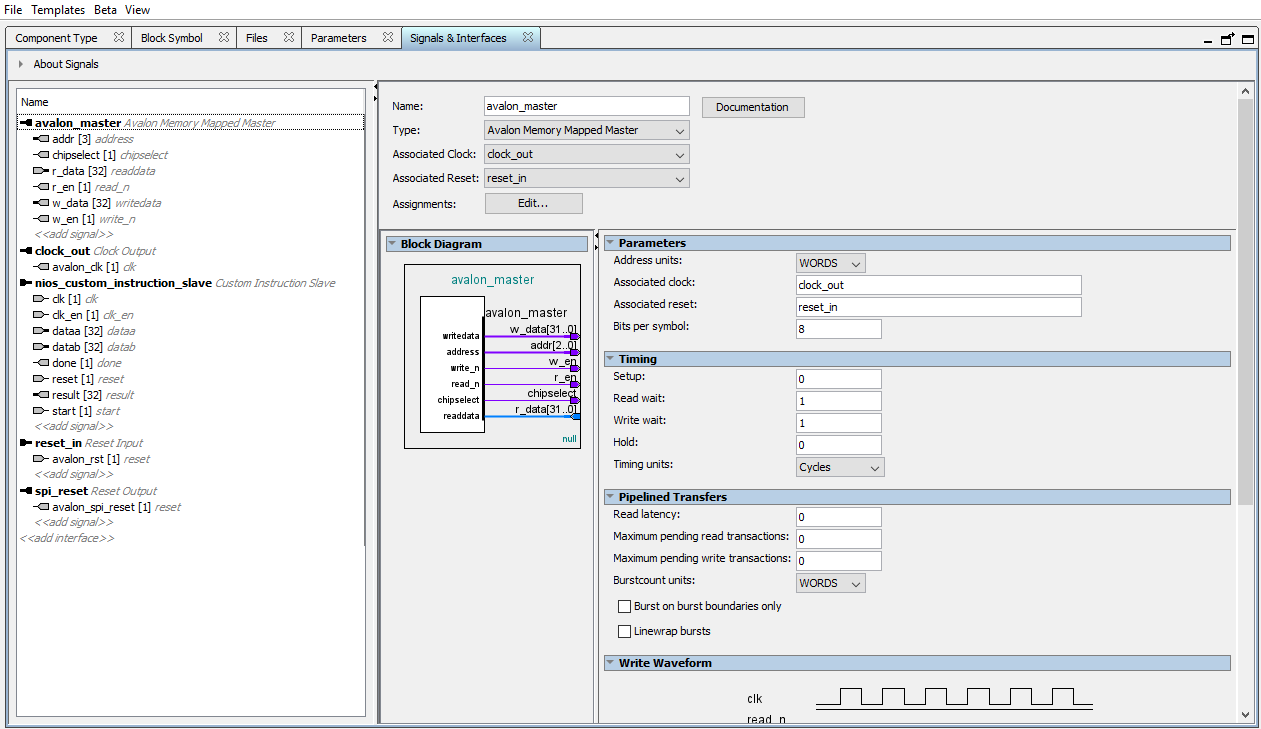
\includegraphics[width=1\textwidth]{05_evaluation/images/pd_interfaces.png}
    \caption{Platform Designer: Complete interface \& signal list for the custom hardware}
    \label{fig:pd_interfaces}
\end{figure}

Once all the signal are added, the user will need to click on the “avalon\_master” interface and set the “Address Units” to “WORDS” and the “Write wait” to “1”, shown in \autoref{fig:pd_avalon}. They will also need to select the “clock\_out” interface and set the “Clock rate” to “50000000” and enable “Clock rate known”, refer to \autoref{fig:pd_clock}.

\begin{figure}[!htb]
    \centering
    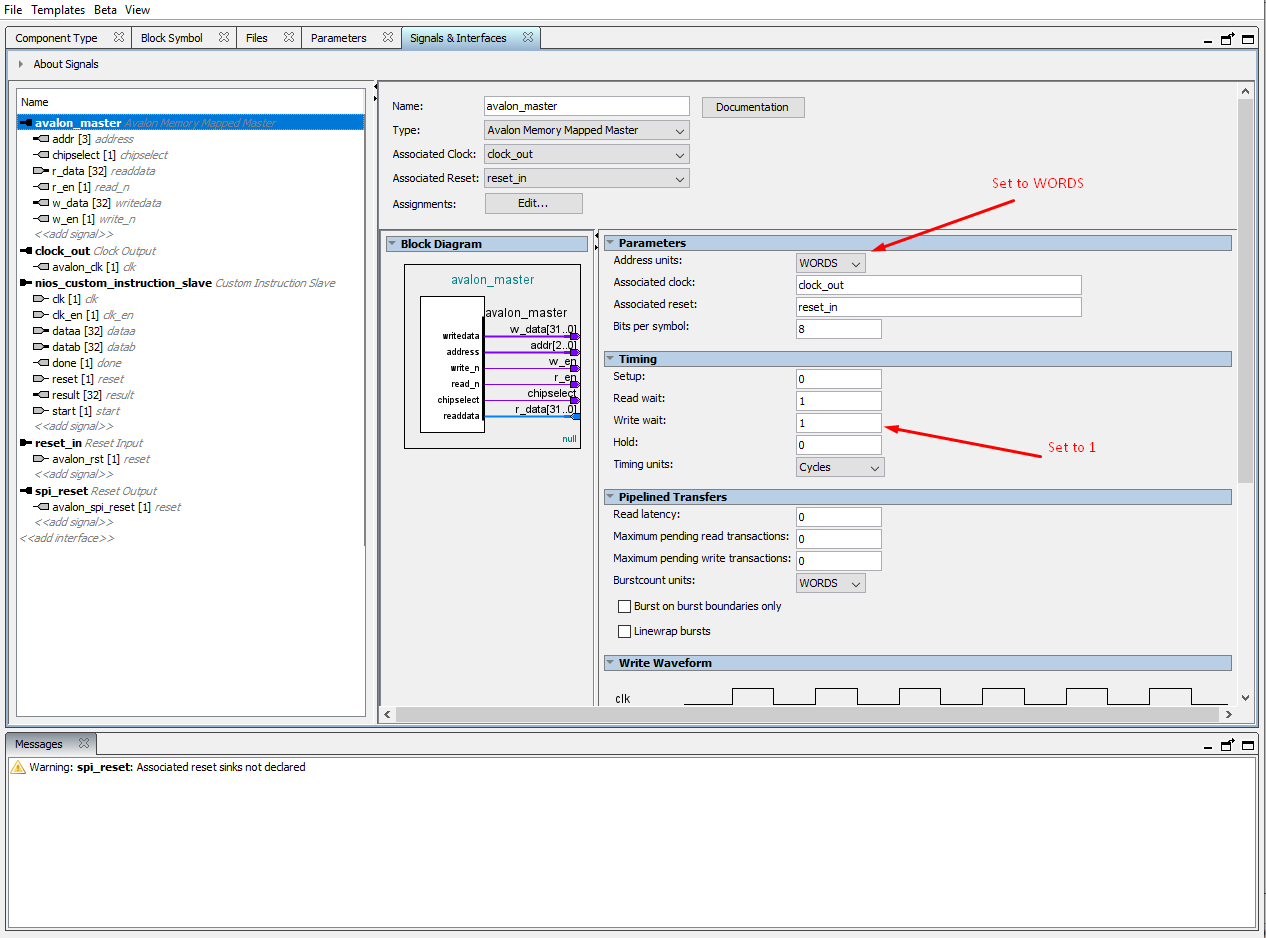
\includegraphics[width=1\textwidth]{05_evaluation/images/pd_avalon_config.png}
    \caption{Platform Designer: Avalon config}
    \label{fig:pd_avalon}
\end{figure}


\begin{figure}[!htb]
    \centering
    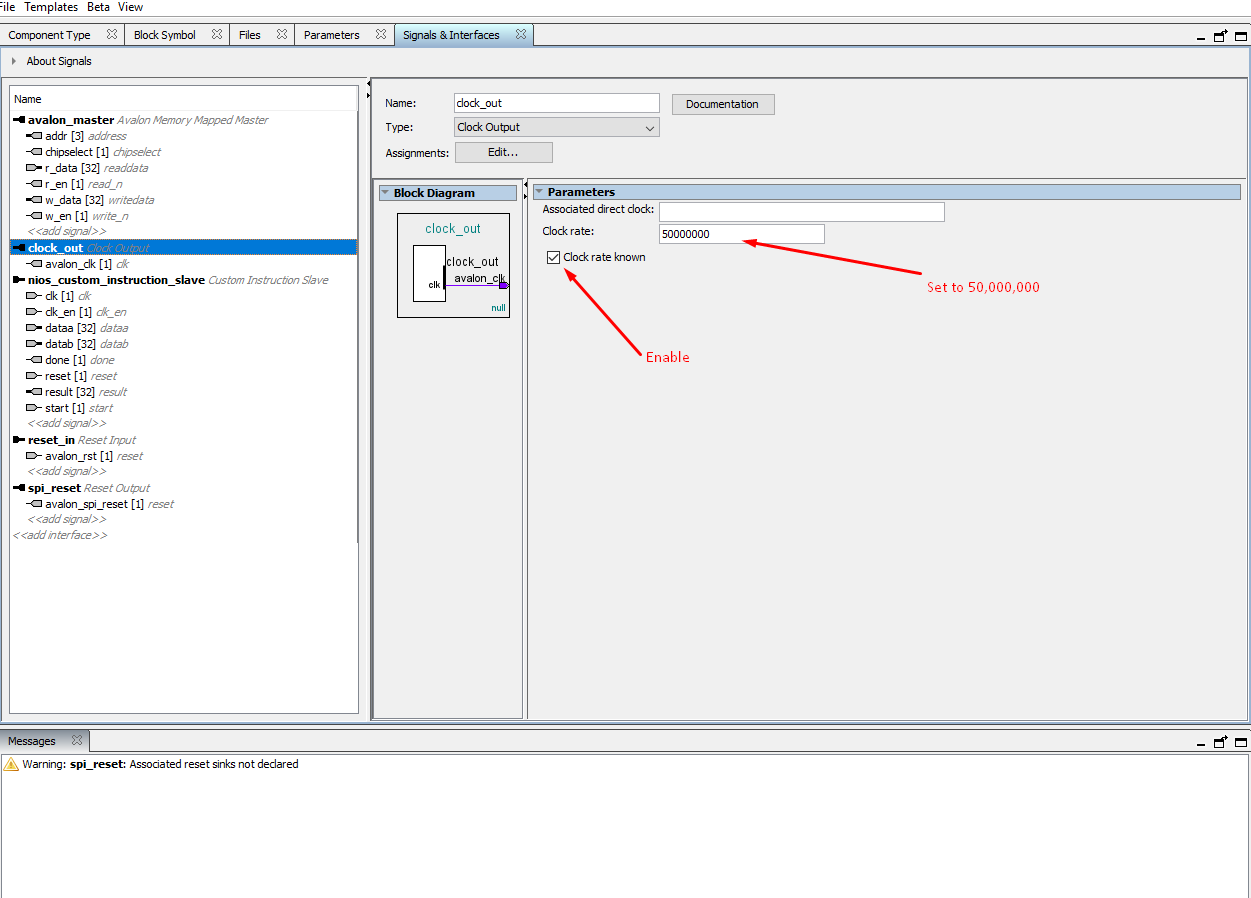
\includegraphics[width=0.9\textwidth]{05_evaluation/images/pd_clock.png}
    \caption{Platform Designer: Clock output config}
    \label{fig:pd_clock}
\end{figure}

A user may then click “Finish...” to save their design and exit out of the “Component Editor”. Now that their module has been added to the catalog, a user can search for their custom hardware and add it to their system. Once their module has been added, they will need to connect it to the other modules in the system. The important modules are “CPU” and “spi\_0”. The first represents the NIOS II processor, and we connect it to our module through the Custom Instruction” interface. The “spi\_0” is an IP core provided by intel to interface with an SPI channel. This module will be driving the GPIO pins, while the user's custom hardware will be controlling it and providing it data.

To connect the custom hardware module, click on the dots shown in \autoref{fig:pd_connections}. They should be empty white circles initially, and then should fill when enabled. The user should then save the system and click “Generate HDL”. In the prompt that shows up, most default settings should be kept however the user should make sure “Create block symbol file (.bsf)” is enabled. “Generate” can then be clicked and in the “Platform Designer” window the user can press “Finish” to exit the tool.

\begin{figure}[!htb]
    \centering
    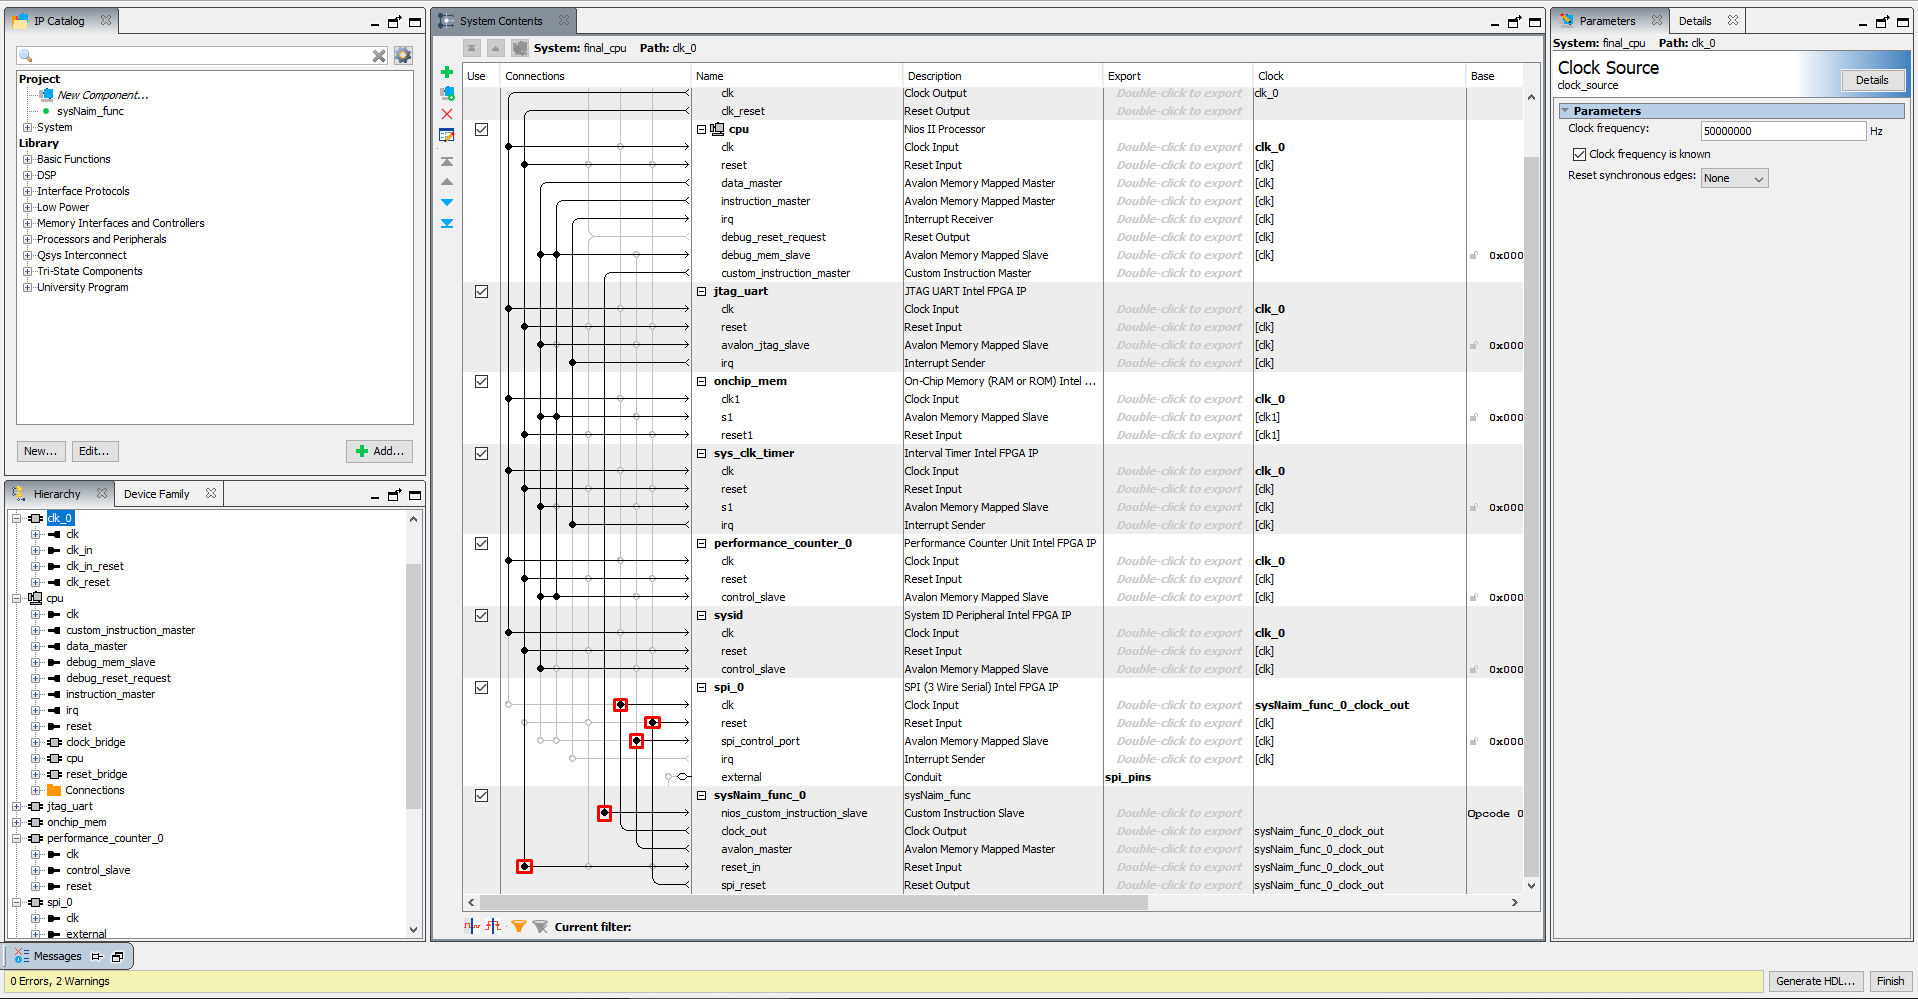
\includegraphics[width=0.9\textwidth]{05_evaluation/images/pd_connections.png}
    \caption{Platform Designer: Connections to the custom hardware}
    \label{fig:pd_connections}
\end{figure}

\subsubsection{Back to Quartus}

Once back in Quartus, the user will need to add the “parent\_cpu.qsys” file to the project files. They can then add their system, which will be named “parent\_cpu”, to the top-level file containing the pins. Wire up the pins to their appropriate ports on the CPU module, as shown in \autoref{fig:qp_connected}. Then add a VCC block and connect it to the “reset\_n” port. The user may then synthesize the top-level file and load it onto the FPGA.

\begin{figure}[!htb]
    \centering
    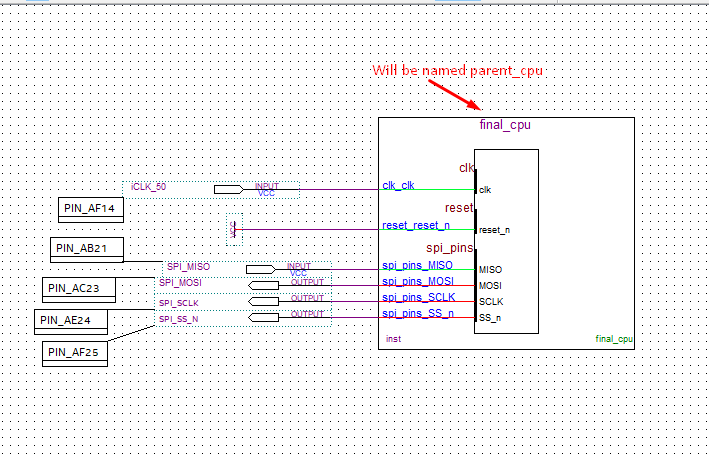
\includegraphics[width=0.9\textwidth]{05_evaluation/images/qs_cpu_connected.png}
    \caption{Quartus Prime: NIOS System connected to pins in top-level file.}
    \label{fig:qp_connected}
\end{figure}

\subsubsection{NIOS II Eclipse}

The final tool the user will need to use is the NIOS II Software Build Tools for Eclipse. It is recommended that the user read the following: pages 4-7 of “My First NIOS II Software” \cite{nios-ii-first-prog} and chapter 3 of “NIOS II Custom Instruction User Guide” \cite{nios-ii-inst-guide}.

Once the user understands how to create a NIOS II project and call custom instructions they can run their own custom hardware on their FPGA.

Example code files for both the child and parent FPGA can be found in Listings \ref{lst:parent_code} and \ref{lst:parent_code} respectively.

\subsubsection{Child FPGA Setup}

The sections starting from opening up Quartus will need to be repeated in order to set up the user's child FPGA. When performing these steps again most are the same, except when in the “Platform Designer”, the user should open up the “child\_cpu.qsys” file instead. They must also set the “sysNaim\_remote\_top.sv” as the top-level file, and include the hardware files in the “child\_fpga” folder instead of the “parent\_fpga” folder. Calling the function in NIOS II for Eclipse will be the same except that the function name will be different.

\subsubsection{Running the System}

Before the bitstreams are downloaded onto the FPGAs, the user should first connect the GPIO pins they assigned names to. So the SPI\_MISO pin on the parent FPGA should be connected to the SPI\_MISO pin on the child FPGA, and so on for all the other SPI pins. One this is done the FPGAs can be programmed, ready for the systems to be run.

To run the system, the child FPGA starts first so that it is ready to receive a transaction from the parent FPGA. Once the child FPGA has been started, the parent FPGA can be run. When the NIOS II terminal displays the result, the system has completed operation.

\subsection{Creating a Multi-FPGA System from Scratch}
\label{sec:scratch}

Going through a step-by-step design example for implementing a multi-FPGA system would likely take an obscene amount of pages and would do very little to showcase the main differences in complexity between such a system and one implemented using SystemNaim. Instead, the following sections will provide an overview of the main challenges and considerations that one would have to think about if they were to create a system just using Quartus Prime and SystemVerilog.

Afterwards, a comparison will be made of performing the same task using SystemNaim. Both the benefits and disadvantages for both solutions will be given to provide a fair and a balanced evaluation.

\subsection{Computing the Result.}
\label{sec:dedicated_hardware_computation}

The first task a user would have to complete is designing the system which computes their desired function. Unlike programming in software, designing in hardware requires a full understanding of the system before any HDL is written.

As an example, let us consider a module which computes the value for a function, $f(x)$. A user must consider design decisions such as, is this module combinational or sequential? Is a ready signal necessary to tell a connected module whether this module is ready to take in data? Will I assume all modules connected to this one know the latency of this module, or will there be a done signal?

Before the computation within the module is reasoned about, a user must decide how this module will be used by the hardware blocks connected to it. The interfaces of a module are of key importance since they determine how a module accepts data and how it should output data once it has finished computation.

Even when we can start writing the hardware logic, the paradigm shift from software programming becomes larger. For loops don't necessarily exist in Verilog the same way as normal programming languages. To implement something similar a state machine, whose computation resembles a for loop written in assembly, must be designed. However, this may not be the most optimal solution, and instead, having a FIFO as an interface input and grabbing data from it when it is available would be a better way of iterating over data. The latter solution is something very few people, outside those with experience in concurrent programming and queues, would think to implement, but it would result in a more streamlined system with less overhead states.

In comparison to software programming, hardware design requires a user to put much more thought into how the modules connect rather than just what their computations consists. A single mistake in deciding which cycle to pass data from one module to another can cause a cascade of failures, resulting in the entire system being rendered useless. Even debugging is more difficult, you can't merely call your main function with some inputs and print to console in places you think the program is broken. Instead, you have to simulate your entire design, including manually creating valid transactions for you top level module, and then find the issue by following incorrect wire or register values to their source.

\subsubsection{Comparison to SystemNaim}

When creating a system in SystemNaim, it's exactly the same as developing software. You can write a program in C and trust that the tool will create the correct hardware which computes the same result. The main draw of HLS is that a user no longer needs to worry about timing violations or what number states are necessary for this module, instead they can focus on the actual computation which the system needs to implement. Creating dedicated hardware to compute the Composite Simpson numerical integration would likely take a few hours, but in SystemNaim it only takes 15 minutes. This speed-up in development time is crucial for implementing larger systems in hardware within a reasonable time frame and is one of the major contributions we say SystemNaim achieves in \autoref{sec:contributions}.

However, the increase in user productivity does come at cost. The output Verilog will likely have much worse latency than hardware designed for a specific system. If an individual were to create dedicated hardware to compute the Composite Simpson numerical integration, the latency would be much lower than the system created in SystemNaim. Therefore, a user must decide if the increase in latency of the resulting hardware is worth the reduction in development times. For larger systems this potentially may be the case as it would be otherwise unfeasible to create all the hardware manually.

\subsection{Converting to Multi-FPGA}

The main purpose of SystemNaim is to streamline the process of creating a multi-FPGA system. But, what issues and challenges would one face if they decided to create a multi-FPGA system using only Quartus and Verilog. Firstly they would have to decide how the two FPGAs would communicate with each other. Usually this is done over a communication channel such as SPI which then begs the question: whether they would want to use Intel's SPI core, or any other communication IP core, to control their channel or create their own hardware. The latter is ill-advised unless they wish to create their own protocol, but the former usually requires an understanding of an Intel designed interface.

In the case of the Intel SPI core, there is an Avalon-MM interface, which requires the user to control signals such as: address, read data, write data, read/write enable, and chipselect. All signals have their own purpose and misunderstanding any of their uses leads to an inability to interact with the core. Therefore, in order to use one of these cores a user has to design a hardware module which correctly interfaces with the core so that they are able to send and receive data over the channel. Sometimes, the provided core on the child FPGA may have a slightly different implementation, which requires an additional hardware module to be created in order to interface with it correctly.

But once the required interfacing hardware is created, the user must then decide what data they wish to send over. Sending more data over the channel allows for more processing to occur on the child FPGA, however this incurs a latency cost as explored in \autoref{sec:interconnect} and thus sending too much data will slow down the system. On the other hand, sending too little data will reduce the amount of processing that can be done on the child FPGA as it won't have anything to actually process. Potentially, the designer could only use the communication channel to send commands to the off-chip and not any actual data. This would mean that all data would need to created on the child FPGA, or known by it at compile time, thus drastically reducing its versatility at run-time. Using the Composite Simpson example once again, the designer could decider that the values of $a$, $b$, $n$, and $h$ are never going to change and thus no data needs to be sent to the child FPGA when it's computing its sum. However, this would mean that if the user wanted to integrate over a different part of the function they would need to recompile the entire system. 

The resulting decision ends up being a balance between being able to compute as much as possible on the child FPGA and not incurring too much of latency cost from using the communication channel, but a user can tailor it to their specific needs.

The next issue the user faces is connecting this communication channel to their main system. Assuming they have decided what data is being sent over and what processing is occuring on the child-FPGA they will then need to create a new data path to send the correct data to the communication channel. They will then need to decide if they want to wait for the processing off-chip to be finished before they continue any other operation or if they would like to perform some computation on the parent FPGA in parallel. The latter is strongly advised, but requires additional hardware to wait for both data paths to finish processing.

If the system has already been designed with parallelism in mind, and the user wished to offload one of the parallel data paths to the child-FPGA, then the new data path will likely just be a modification of a pre-existing one. If the system had no parallelism beforehand, then creating a new data path may require an entire overhaul.

Overall, creating a multi-FPGA system is not just about setting up a communication channel but rather considering which parts of the system would benefit from being processed off chip, and what data those parts require. But it is still a tedious and long process to create a functioning communication channel.

\subsubsection{Comparison to SystemNaim}

In SystemNaim, we use function calls as a method of allowing the user to decide what processing occurs off and on-chip. This makes it much easier for new users to split their program across multiple FPGAs, which is a requirement of the HLS tool specified in \autoref{sec:hls_design}. They don't have to worry about interfacing correctly with the SPI core, or creating a new data path to accommodate for the off-chip processing. Instead, they can treat it as a normal function call and nothing more. Of course, following from \autoref{sec:sys_perf}, there are recommendations that the user should follow when creating their program, but they are free to explore designs as they wish, and they can experiment with choosing which parts of their program to process off-chip without having to go through the hassle of re-hauling their entire system, if they had chosen to do it manually.

It goes without saying, though I will say it, that there aren't only advantages to using SystemNaim. The user is limited to only being able to design functions with two inputs, which does limit the potential use cases. If they had designed their own hardware system, they would be able to transmit as much data as possible. SystemNaim also forces each transaction across the channel to be 32 bits long, in order to ensure a full integer can be sent across. However, some systems may not need to full 32 bits which results in unneeded additional latency.

Once again, the decision to use SystemNaim or not is a balance between latency and development time. A manually designed system, focusing on one application, will be faster and will use less resources. But, it may take much longer to create. When creating SystemNaim it took us a week to create the hardware to control communication channel and even longer to debug it. Therefore, I would posit, that even though it may result in latency increases, the time saved from using SystemNaim, and any HLS tool derived from it, will allow for much larger systems to be created and for more experimentation on multi-FPGA platforms to take place.

\subsection{Conclusion}

The sections above show that while SystemNaim does create less optimized systems, than dedicated hardware, it does streamline the development process and reduce the time taken to get a system running, which is one of the primary contributions mentioned in \autoref{sec:contributions}. To further illustrate this two example project timelines are shown in Tables \ref{tbl:time_sysNaim} and \ref{tbl:time_custom}. As a disclaimer, these values have been chosen from my own experience, they may vary from person to person, and external factors may also affect, for example if the FPGA had a hardware defect and extra time was spent debugging that. The durations stated in \autoref{tbl:time_sysNaim}, assume the user is following the design example above for the first time, and have no knowledge of their FPGA's pin layout. The overhead times can decrease greatly as the user becomes more proficient in these tools, leaving only the development as the main contributing factor. \autoref{tbl:time_custom} assumes the individual implementing the system has an amount of experience with hardware development close to ours, as the time values are an estimate of how long it would take us to implement these parts. We also have assumed that the system design already accounts for off-chip processing, and no overhaul is required when reaching the implementation of the channel starts. Finally, it should be noted that a large part of the time spent is mostly in design and debugging rather than the writing of HDL.

From these tables we can see that SystemNaim would save a designer, days in development time and this would be for a relatively simple system. Larger systems take even longer to design in Verilog and Quartus, but the increase in time for SystemNaim or other HLS tools would be far less. Therefore, with some leniency, it can be concluded that we have proved our 3rd contributions specified in \autoref{sec:contributions}.


\begin{table}[]
\begin{tabular}{l|l|l}
Task                                 & Time Spent & Cumulative Time Spent \\ \hline
Programming System                   & 1h         & 1h                    \\
Creating System in Platform Designer & 30m        & 1h 30m                \\
Assigning Pins in Quartus            & 1h         & 2h 30m                \\
Setting up NIOS II environment       & 1h         & 3h 30m               
\end{tabular}
\caption{Time to taken to create a multi-FPGA system in SystemNaim, assuming beginner FPGA knowledge.}
\label{tbl:time_sysNaim}
\end{table}


\begin{table}[]
\begin{tabular}{l|l|l}
Task                               & Time Spent & Cumulative Time Spent \\ \hline
Implementing Computational System  & 3d         & 3d                    \\
Implementing Communication Channel & 3d         & 6d                    \\
Overhead using tools               & 2h         & 6d 2h                
\end{tabular}
\caption{Time to taken to create a multi-FPGA system in with just Verilog and Quartus, assuming intermediate FPGA knowledge.}
\label{tbl:time_custom}
\end{table}


One last note that is important to this analysis, regards to the steps shown in \autoref{sec:design_example}. Many of the steps shown when setting up a SystemNaim system are not related to the development of the program, but rather they illustrate the overhead that comes with getting it to run. Tasks such as; finding a way to control the system, connecting the program hardware to the SPI core, assigning pins to use as the communication channels, would still be present if a user decided to implement their own system from scratch. Potentially the steps regarding NIOS II could be avoided, but then additional effort would be needed to find a way of controlling and testing the system. In addition, pre-made files which streamline these tasks would also not be available and the designer would have to gain a deeper understanding of all the aforementioned tools to complete their system. Therefore, SystemNaim can be said to not only quicken the development process but also the process of getting the system actually running on an FPGA.







